%CAPITULO 4a
%pagina 23
\begin{frame}{Optimidad de A* (prueba estándar)}
Supongamos que se ha generado un objetivo subóptimo \textcolor{purple}{$G_{2}$} y está en la cola. Sea \textcolor{purple}{$n$} un nodo no expandido en el camino más corto hacia un objetivo óptimo \textcolor{purple}{$G_{1}$}. \\
\centering
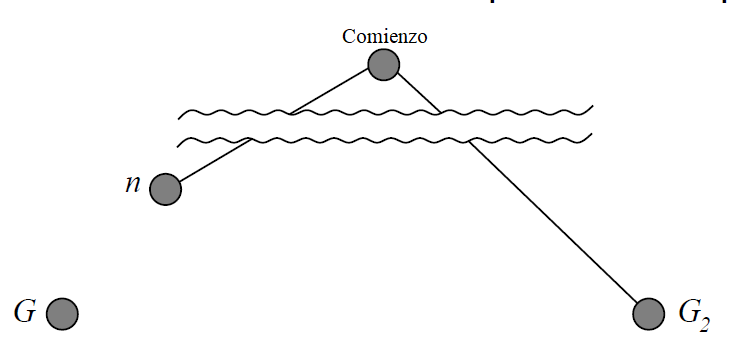
\includegraphics[scale=0.3]{images/23_image_ca4a3pag23.png}
 \begin{flushleft}
$f(G_{2}) = g(G_{2})$ ya que $(G_{2}) = 0$\\
\hspace{1cm}$> g(G_{1})$ ya que $G_{2}$ es subóptimo\\
\hspace{1cm}$\geq f(n)$ ya que $h$ es admisible\\
\vspace{5mm}
\end{flushleft}
Ya que $f(G_{2})> f(n)$, A* nunca seleccionará $(G_{2})$ para expansión.
\end{frame}